\chapter{Разработка нового нейросетевого подхода} \label{ch2}
	
% не рекомендуется использовать отдельную section <<введение>> после лета 2020 года
%\section{Введение} \label{ch2:intro}

Существующие решения, решающие задачу автофокусировки микроскопа, показывают хорошие результаты, но их главный минус в том, что они не являются универсальными. В этой главе будет рассказано о новом подходе на основе машинного обучения, который не требует никаких особых датчиков и интеграции в ПО камеры.

\section{Основные требования к разрабатываемому подходу} \label{ch2:title-abbr} %название по-русски

Сложность развертывания и применения решений на основе фазовых изображений побудила к разработке нового алгоритма, который не имеет такого количества ограничений и недостатков. Таким образом получаем следующие основные пункты, которые нужно учесть при разработке:

\begin{enumerate}[1.]
	\item На вход должно подаваться изображение с камеры. Алгоритм не должен задействовать какие-либо датчики системы регистрации, которые могут отсутствовать на большинстве видов аппаратуры. Поэтому самым удобным и очевидным входным параметром является изображения.
	\item Алгоритм должен принимать на вход ровно один снимок. Если для расчета фокальной плоскости будет использовать набор изображений, то алгоритм будет работать недостаточно быстро, так как скорее всего потребуется многократное смещение камеры в некоторые промежуточные позиции.
	\item Алгоритм должен определять не только величину смещения линзы/камеры, но и его направление. Это также необходимо для достижения максимальной скорости работы.
\end{enumerate}

\section{Элементы нейронных сетей}
В данной работе ключевое место имеет подход к задаче автофокуса на основе глубокого обучения. Нейронные сети, которые позволяют работать с изображениями и извлекать различные важные признаки из них, имеют ряд конструктивных особенностей. Далее подробно будут рассмотрены элементы, которые будут применены в разработанном нейросетевом методе автофокусировки и требуют особого внимания.

\subsection{Сверточный слой} \label{par:convolution}
\textit{Сверточный слой} -- это слой нейронной сети, который выполняет одноименную математическую операцию. Свертка двух функций можно интерпретировать как меру схожести или корреляции этих двух функций. Формально операция свертки определяется следующим образом:
\begin{equation}
	s(x) = (f*g)(x) \stackrel{\text{def}}{=} \int\limits_{\RR^n} f(y)g(x-y)dy = \int\limits_{\RR^n} f(x-y)g(y)dy,
\end{equation}
где $f,\ g:\RR^n \rightarrow \RR$ -- функции, интегрируемые в смысле Лебега, $s:\RR^n \rightarrow \RR$.

В случае работы с изображениями вместо функций $f \text{и} g$ используются многомерные массивы, как правило, двумерные целочисленные. Исходя из этого, стоит переопределить операцию свертки для дискретизированного набора данных следующим образом:
\begin{equation}
	S(i,j) = (I*K)(i,j) = \sum\limits_m \sum\limits_n I(i-m,j-n)K(m,n),
\end{equation}
где $I$ -- исходное изображение, $K$ -- \textit{ядро свертки}, $S$ -- \textit{карта признаков} или \textit{карта активации}, $(i,j)$ -- её пиксель, $(m,n)$ -- индексы, перебирающие пиксели ядра свертки.

В контексте нейросетей и глубокого обучения вместо операции свертки обычно используется родственная ей операция, которая называется \textit{кросс-корреляцией}. Она симметрична функции свертки и имеет тот же смысл, однако перекрестная корреляция проще и быстрее реализуется, так как не требует отражения ядра свертки по обеим осям. Кросс-корреляция имеет следующий вид:
\begin{equation}
	С(i,j) = (I*K)(i,j) = \sum\limits_m \sum\limits_n I(i+m,j+n)K(m,n),
	\label{eq:cross-correlation}
\end{equation}

Если изображение, подаваемое на вход, является многоканальным (например, формата RGB). В таком случае для каждого канала изображения используется свое ядро свертки. Набор таких ядер называется \textit{фильтром свертки}. При этом таких фильтров может быть несколько. Каждое ядро свертки является обучаемым.

\textit{Свертка по глубине} или \textit{depthwise свертка}. \textbf{[MobileNets: Efficient Convolutional Neural Networks for Mobile Vision Applications]}. Этот тип свертки был предложен в 2016 году, и основная его цель -- это значительное снижение вычислительной нагрузки, а выполняется он в два этапа. На первом этапе, в отличие от стандартной свертки, в свертке по глубине для каждого канала входного тензора используется свое ядро свертки. Таким образом, фильтр depthwise свертки для цветного трехканального изображения будет состоять из трех ядер и на выходе после первого шага будет также трехканальный тензор. На втором этапе применяется привычная свертка с ядром размера $1 \times 1$ и с указанным числом фильтров, чтобы собрать полученную информацию по признакам в единое целое.

Благодаря такому подходу, вычислительная сложность алгоритма и количество обучаемых параметров значительно уменьшаются, что очень важно, когда алгоритм применяется в условиях ограниченности времени или мощностей \textbf{[тот же источник, стр 2-3]}.

\textit{expansion/dilated}


\subsection{Функции активации}
В этой работе используется несколько

\subsection{SE блоки}
\textit{Squeeze-and-Excitation (SE) блок} -- это архитектурное дополнение к сверточным слоям, главная цель которого -- улучшение производительности путем отбора признаков, наиболее сильно влияющих на результат. SE блоки перенастраивают веса, усиливая значимые признаки и подавляя менее важные. В предлагаемой нейросети SE блок имеет структуру, изображенную на \firef{fig:SE_block}. Такой блок обрабатывает данные в три шага:
\begin{enumerate}[1.]
	\item Сжатие (Squeeze). На это этапе происходит глобальное объединение по среднему (global average pooling) на каждом канале входного изображения, сжимая пространственные показатели признаков в одно число. Это позволяет извлечь глобальную информацию с о канале.
	
	\item Возбуждение (Excitation). Этот шаг объединяет в себе несколько слоев. Сначала используется полносвязный слой с функцией активации ReLU, зачет еще один полносвязный слой с логистической функцией активации (сигмоидой). Первый слой уменьшает количество каналов с $C$ до $C/r$, где $r$ -- некоторый коэффициент. В большинстве случаев его принято устанавливать равным 16. Второй слой восстанавливает исходное количество каналов. Такой процесс позволяет улавливать и моделировать взаимосвязи между каналами. Кроме того, механизм понижения и восстановления размерности действует как регуляризация и уменьшает возможность переобучения. Стоит отметить, что на практике (например, в библиотеке Pytorch) чаще встречаются реализации SE блоков с использованием свертки с ядром $1 \times 1$ вместо полносвязных слоев. Это обусловлено тем, что в таком случае сохраняется пространственная структура, что позволяет более естественно и удобно работать с многомерными данными, коими являются изображения и результаты применения сверточных слоев. То есть не приходится выравнивать многомерный массив (такая операция называется \textit{flattening}). А также применения свертки более эффективно с точки зрения вычислений и памяти, так как графические и тензорные процессоры оптимизированы для выполнения именно этой операции, и их ресурсы будут расходоваться экономичнее.
	
	\item Перенастройка весов (Reweight). Весовые коэффициенты, полученные на прошлом этапе, поэлементно умножаются на исходные признаки.
\end{enumerate}

\begin{figure}[ht] 
	\center
	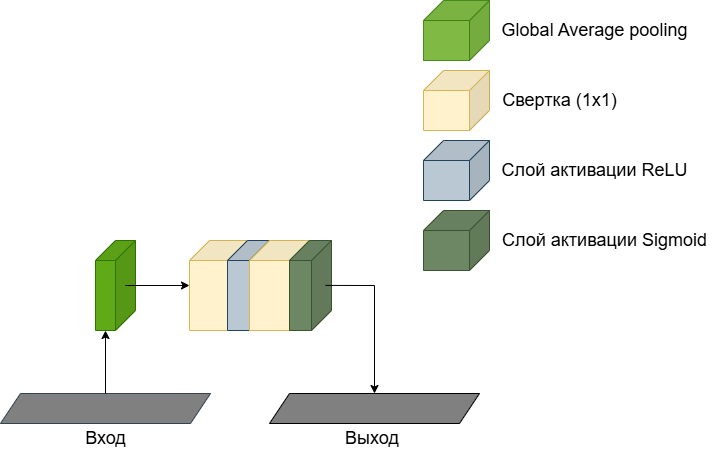
\includegraphics [scale=0.5] {my_folder/images/FocusNet-SE layer.png}
	\caption{Squeeze-and-Excitation блок}
	\label{fig:SE_block}
\end{figure}

\section{Архитектура нейросети}

В основе разработанного решения лежит сверточная нейросеть MobileNet от Google, которая была разработана для классификации объектов на изображении на смартфонах. Существует несколько модификаций данной нейросети. Для решения задачи автофокуса бьла выбрана версия MobileNetV3\_Small. Одним из ключевых факторов в принятии решения была скорость работы и легковесность, так как принимать решение о смене позиции камеры нужно максимально быстро, не затрачивая больших вычислительных ресурсов.

Главная идея аданной сети -- так называемые bottleneck-блоки. Они используют depthwise свертку, преимущество которой заключается в снижении вычислительной нагрузки благодаря меньшему количеству операций и меньшем числе обучаемых параметров. В следствие этого уменьшается время обработки входных данных нейросетью, а сам алгоритм становится менее требователен к оборудованию в условиях ограниченных мощности и памяти.

Далее были внесены некоторые изменения в архитектуру MobileNet, чтобы адаптировать ее для решения поставленной задачи. Изменилась сама цель алгоритма: если оригинальная сеть предназначалась для классификации, то модифицированная версия для автофокуса должна решать задачу регрессии, так как ее цель -- предсказание непрерывной величины, а именно смещения камеры. В данном случае набором признаков (или факторов) для предсказания данной величины является само входное изображение.

Для того, чтобы адаптировать алгоритм под задачу регрессии, необходимо было внести изменения в последние слои, заменив классификатор на последовательность слоев, выполняющих регрессию. Классификатор состоял из двух полносвязных слоев, функции активации hardswish, слоя исключения (далее dropout или дропаут). Регрессор же состоит из двух полносявзных слоев и функции активации ReLU.

В качестве функции потерь была выбрана smooth L1-loss, которая является комбинацией L1-loss, также известной как Mean Absolute Error (MAE) или средняя абсолютная ошибка, и L2-loss -- Mean Squared Error (MSE) или средней-квадратичной ошибкой. Smooth L1-loss задается следующей формулой:
\begin{equation}
	L1_{smooth} =
	\begin{cases}
		\dfrac{1}{2\beta}(y-y')^2,\ |y-y'|<\beta \\
		|y-y'| - \dfrac{\beta}{2},\ \text{иначе}
	\end{cases},
\end{equation}
где $y$ -- истинное искомое значение, $y'$ -- предсказанное значение, $\beta$ -- некоторая константа, которая задается при настройке сети и в данном случае равная единице. Выбранная функция потерь имеет следующие преимущества:
\begin{enumerate}[1.]
	\item Стабильность градиента. Smooth L1-loss малых ошибок ведет себя как MSE, а для больших -- как MAE. Константа $\beta$ задает величину ошибки, на которой происходит это разделение. Но как известно, градиент функции L1-loss не определен в нуле, из-за чего могут возникать трудности при обучении во время обратного распространения ошибки. Вероятность совпадение истинного и предсказанного значений мала, но все же такое случается. Градиент функции средне-квадратичной ошибки лишен этого недостатка, но эта функция потерь вносит слишком большое влияние при больших ошибках. Градиент функции smooth L1-loss выглядит следующим образом:
	\begin{equation}
		\nabla L1_{smooth} = 
		\begin{cases}
			\dfrac{y-y'}{\beta},\ |y-y'|<\beta \\
			\text{sign}(y-y'),\ \text{иначе}
		\end{cases}
	\end{equation}
	
	Это способствует лучшей сходимости алгоритма обучения.
	
	\item Устойчивость к выбросам. Функция потерь MSE чувствительна к выбросам из-за квадратичной зависимости от ошибки. Smooth L1 при больших отклонениях ведет себя линейно, что позволяет избежать слишком большого влияния ошибок.
\end{enumerate}

Таким образом, Smooth L1-loss является некоторым симбиозом функций абсолютной и среднеквадратичной ошибки, вобрав в себя лучшее от каждой из них.

Описание архитектуры нейросети представлено в \taref{tab:nn_architecture}. Более детальную схему слоев можно увидеть на \firef{fig:FocusNet}. 

\begin{table}[!htbp]
	\centering
	\small
	\begin{tabular}{|c|c|c|c|c|c|c|}
		\hline
		Вход & Слой & exp size & Выход & SE & AF & stride\\ \hline
		$672^2 \times 3$ & conv2d, $3 \times 3$ & - & 16 & - & Hardswish & 2\\ \hline
		$336^2 \times 16$ & bneck, $3 \times 3$ & 16 & 16 & \checkmark & ReLU & 2\\ \hline
		$168^2 \times 16$ & bneck, $3 \times 3$ & 72 & 24 & - & ReLU & 2\\ \hline
		$84^2 \times 24$ & bneck, $3 \times 3$ & 88 & 24 & - & ReLU & 1\\ \hline
		$84^2 \times 24$ & bneck, $5 \times 5$ & 96 & 40 & \checkmark & Hardswish & 2\\ \hline
		$42^2 \times 40$ & bneck, $5 \times 5$ & 240 & 40 & \checkmark & Hardswish & 1\\ \hline
		$42^2 \times 40$ & bneck, $5 \times 5$ & 240 & 40 & \checkmark & Hardswish & 1\\ \hline
		$42^2 \times 40$ & bneck, $5 \times 5$ & 120 & 48 & \checkmark & Hardswish & 1\\ \hline
		$42^2 \times 48$ & bneck, $5 \times 5$ & 144 & 48 & \checkmark & Hardswish & 1\\ \hline
		$42^2 \times 48$ & bneck, $5 \times 5$ & 288 & 96 & \checkmark & Hardswish & 2\\ \hline
		$21^2 \times 96$ & bneck, $5 \times 5$ & 576 & 96 & \checkmark & Hardswish & 1\\ \hline
		$21^2 \times 96$ & bneck, $5 \times 5$ & 576 & 96 & \checkmark & Hardswish & 1\\ \hline
		$21^2 \times 96$ & conv2d, $1 \times 1$ & - & 576 & - & Hardswish & 1\\ \hline
		$21^2 \times 576$ & avgpool2d, $7 \times 7$ & - & 576 & - & - & 1\\ \hline
		$576$ & fully-connected & - & 256 & - & ReLU & -\\ \hline
		$256$ & fully-connected & - & 1 & - & - & -\\ \hline
	\end{tabular}
	\caption{Структура слоев предлагаемой нейросети}
	\label{tab:nn_architecture}	
\end{table}

\begin{figure}[ht] 
	\center
	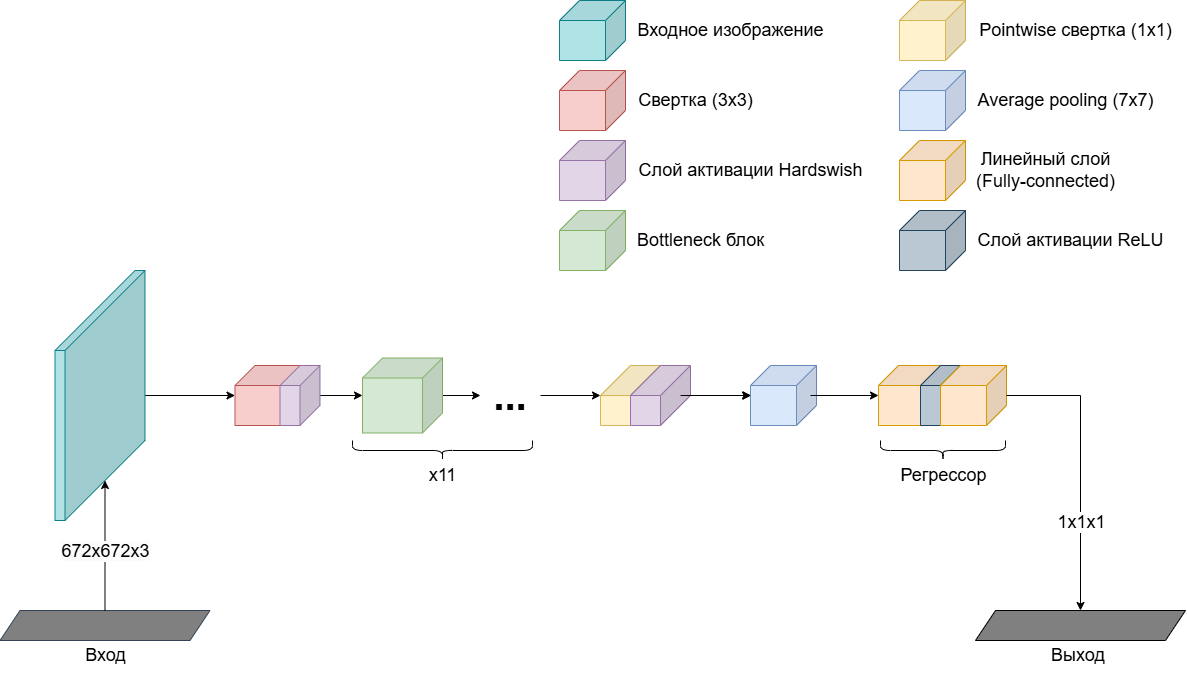
\includegraphics [scale=0.4] {my_folder/images/FocusNet-FocusNet2.png}
	\caption{Общая схема нейросети} 
	\label{fig:FocusNet}
\end{figure}

Также на \firef{fig:FocusNet-Bottleneck} представлена стуктура Bottleneck блока. Данный тип элемента можно считать ключевой инновацией, поскольку в нем используются инвертированные остаточные блоки. Особенность таких bottleneck блоков заключается в следующем:
\begin{itemize}
	\item Инвертированная структура. В традиционных остаточных блоках используется уменьшение размерности данных перед обработкой. В инвертированных блоках сначала происходит увеличение размерности, затем обработка данных, а потом сжатие обратно к исходной размерности. Это позволяет выявлять высокоуровневые признаки в условиях ограниченности вычислительных ресурсов.
	
	\item Свертка по глубине. Как уже говорилось в параграфе \ref{par:convolution}, depthwise свертка значительно уменьшает вычислительную сложность и количество обучаемых параметров.
	
	\item Squeeze-and-Excitation (SE) блоки. Эти блоки помогают адаптивно перенастраивать весовые коэффициенты каналов, усиливая важные признаки и подавляя менее значимые, что улучшает представление данных и общую производительность модели.
	
	\item Функция активации Hardswish. Эта функция проста в вычислительном смысле, помогает нейросети справляться с ленилейными зависимостями, хорошо сохраняет информацию и градиенты при отрицательных значениях входных данных.
\end{itemize}

\begin{figure}[ht] 
	\center
	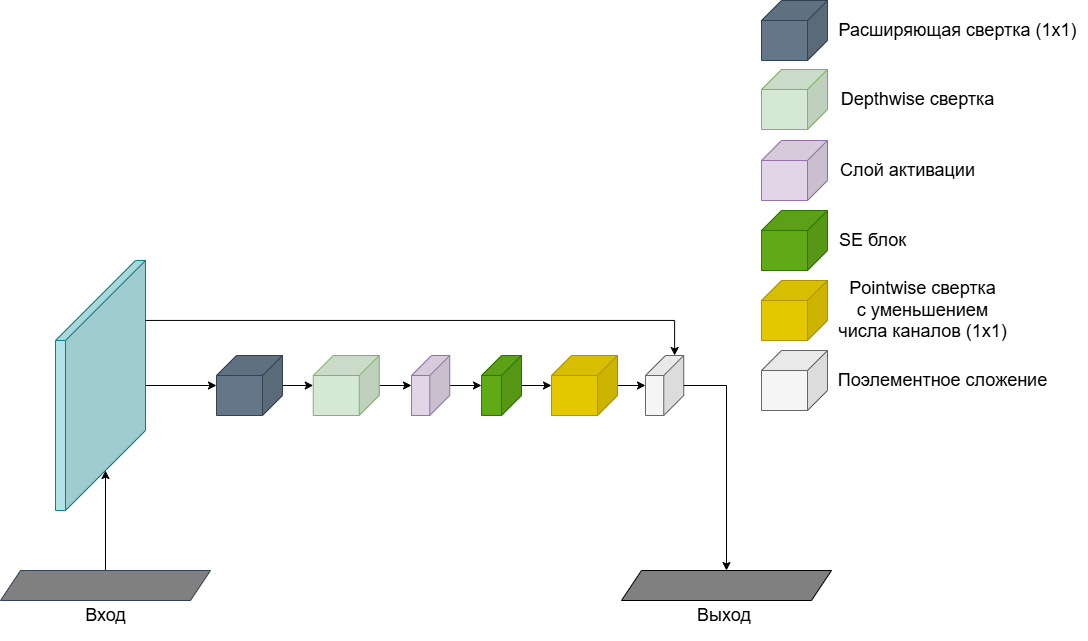
\includegraphics [scale=0.4] {my_folder/images/FocusNet-Bottleneck.png}
	\caption{Структура bottleneck блока}
	\label{fig:FocusNet-Bottleneck}
\end{figure}

\section{Определение направления смещения}
Попытка смоделировать размытое изображение (например, для обучения нейросети) с помощью простых инструментов таких, как размытие по Гауссу, приводит к тому, что между изображениями по обе стороны от фокальной плоскости, но на равном удалении нет разницы. Соответственно, в таком случае нельзя определить направление смещения камеры от объекта съемки. Однако реальная дефокусировка устроена сложнее, она содержит асимметричные хроматические и сферические аберрации. Изображение, получаемое с микроскопа в силу неидеальности систем регистрации и оптики , а также физики света является сверткой <<чистого>> изображения и функции рассеяния точки (ФРТ) \textbf{[Sibarita J. B. Deconvolution microscopy //Microscopy Techniques: -/-. – 2005. – С. 201-243.]}. Помимо этого камера вносит свой шум в получаемое изображение. Таким образом, итоговое изображение можно описать формулой:
\begin{equation}
	I'=I \circledast H + N,
	\label{eq:res_img_with_PSF}
\end{equation}
где $I$ -- исходное изображение, $H$ -- ФРТ, $N$ -- шум от системы регистрации, $I'$ -- результирующее изображение.

Благодаря такому механизму, реальные снимки объекта по разные стороны фокальной плоскости будут отличаться. На \firef{fig:PSF} приведена оценка  асимметрии функции рассеяния точки, смоделированной на разных длинах волн и на разном расстоянии от фокальной плоскости. Хорошо видно, что противоположные друг другу изображения неодинаковые. Именно это позволяет определять направление движения камеры.

\begin{figure}[ht] 
	\center
	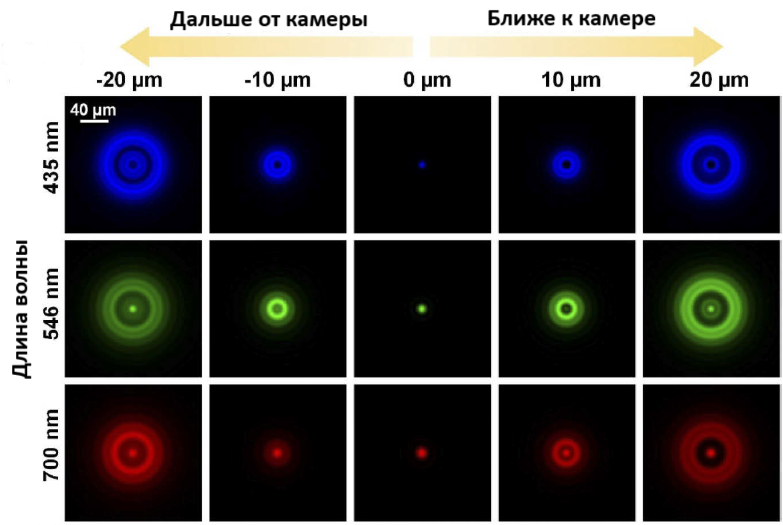
\includegraphics [scale=0.8] {my_folder/images/PSF.png}
	\caption{Смоделированные ФРТ}
	\label{fig:PSF}
\end{figure}

\section{Название параграфа} \label{ch2:sec-abbr} %название по-русски
	
Название параграфа оформляется с помощью команды \verb|\section{...}|, название главы --- \verb|\chapter{...}|. 
	

\subsection{Название подпараграфа} \label{ch2:subsec-title-abbr} %название по-русски


Название подпараграфа оформляется с помощью команды  \texttt{\textbackslash{}subsection\{...\}}.


%\subsubsection{Название подподпараграфа} \label{ch2:subsubsec-title-abbr} %название по-русски
	
Использование подподпараграфов в основной части крайне не рекомендуется. В случае использования, необходимо вынести данный номер в содержание.	
Название подпараграфа оформляется с помощью команды  \texttt{\textbackslash{}subsubsecti\-on\{...\}}.



Вместо подподпараграфов рекомендовано использовать перечисления.

Перечисления могут быть с нумерационной частью и без неё и использоваться с иерархией и без иерархии. Нумерационная часть при этом формируется следующим способом:

\begin{enumerate}[1.]
	\item в перечислениях {\itshape без иерархии} оформляется арабскими цифрами с точкой (или длинным тире).
	\item В перечислениях {\itshape с иерархией} --- в последовательности сначала прописных латинских букв с точкой, затем арабских цифр с точкой и далее --- строчных латинских букв со скобкой. 
\end{enumerate}


%% Если в дальнейшем нужно сделать сслыку на один из элементов нумеруемого перечисления, то нужно использовать конктрукцию типа:

%\begin{enumerate}[label=\arabic{enumi}.,ref=\arabic{enumi}]
%	\item text 1 \label{item:text1}
%	\item text 2
%\end{enumerate}
%\ref{item:text1}.


Далее приведён пример перечислений с иерархией.


\begin{enumerate}
	\item Первый пункт.
	\item Второй пункт.
	\item Третий пункт.
	\item По ГОСТ 2.105--95 \cite{gost-russian-text-documents} первый уровень нумерации идёт буквами русского или латинского алфавитов ({\itshape для определенности выбираем английский алфавит}),
	а второй "--- цифрами. 
	\begin{enumerate}
		\item В данном пункте лежит следующий нумерованный список: 
		\begin{enumerate}
			\item первый пункт;
			\item третий уровень нумерации не нормирован ГОСТ 2.105--95 ({\itshape для определенности выбираем английский алфавит});
			\item обращаем внимание на строчность букв в этом нумерованном и следующем маркированном списке:
			\begin{itemize}
				\item первый пункт маркированного списка.
			\end{itemize}    
		\end{enumerate}
	\end{enumerate}
	\item Пятый пункт верхнего уровня перечисления.
\end{enumerate}

Маркированный список (без нумерационной части) используется, если нет необходимости ссылки на определенное положение в списке:
\begin{itemize}
	\item первый пункт c {\itshape маленькой буквы} по правилам русского языка;
	\item второй пункт c {\itshape маленькой буквы} по правилам русского языка.
\end{itemize} % правила использования перечислений	

	
Оформление псевдокода необходимо осуществлять с помощью пакета \verb|algorithm2e| в окружении \verb|algorithm|. Данное окружение интерпретируется в шаблоне как рисунок. Пример оформления псевдокода алгоритма приведён на \firef{alg:AlgoFDSCALING}. 
	
	
	\begin{algorithm} %[h]
		\SetKwFunction{algoDTestsFDSCALING}{} 
		\SetKwProg{myalg}{Algorithm}{}{} %write in 2nd agrument <<Algorithm>>, <<Procedure>> etc
		\nonl\myalg{\algoDTestsFDSCALING}{
			\KwInput{the many-valued context $\cont[M]\eqdef(G,M,W,J)$, the class membership $\epsilon: G\to K$} 
			\KwOutput{positive and negative binary contexts $\overbar{\cont[K]_+}\eqdef(\overbar{G_+},M,I_+)$, $\overbar{\cont[K]_-}\eqdef(\overbar{G_-},M,I_-)$ such that i-tests found in $\overbar{\cont[K]_+}$ are diagnostic tests in $\cont[M]$, and objects from $\overbar{\cont[K]_-}$ are counter-examples} %последние строки формируют начальное множество диагностических тестов
			\For {$\forall g_i,$ $g_j \in G$\label{step:FD-scaling-first-step}}{
				%(\tcp*[f]{possible inlined comment})
				\If{$i < j$ }{
					$\overbar{G} \leftarrow (g_i,g_j)$\;
				}
			}
			%		$M\leftarrow M\setminus k$\;
			\For {$\forall (g_i,g_j)\in \overbar{G}$}{
				%(\tcp*[f]{possible inlined comment})
				\If{$m(g_i) = m(g_j)$ }{ %на самом деле здесь цикл по всем компонентам вектора-строки
					$(g_i,g_j) I m$\; % or setI() function
				}
				\uIf{$\epsilon(g_i) = \epsilon(g_j)$ }{
					$\overbar{G_+} \leftarrow (g_i,g_j)$\;
				}
				\lElse{$\overbar{G_-} \leftarrow (g_i,g_j)$\label{FD-scaling-step-last}}	
			}		
			$I_+= I\cap (\overbar{G_+}\times M)$, $I_-= I\cap (\overbar{G_-}\times M)$\label{FD-scaling-step-newK}\; 
			\For {$\forall \overbar{g_+}\in \overbar{G_+}$, $\forall \overbar{g_-}\in \overbar{G_-}$ }{
				\If{$\overbar{g_+}\uA \subseteq \overbar{g_-}\uA$ }{
					$\overbar{G_+} \leftarrow \overbar{G_+} \setminus \overbar{g_+}$\;
				}
			}
			%		\Return \;
		}
		\caption{Псевдокод алгоритма \texttt{DiagnosticTestsScalingAndInferring} \cite{Naidenova2017}}\label{alg:AlgoFDSCALING}
		% example of adding an item to Index
		% \index for accepted papers only
		\index[ru]{алгоритм!\texttt{название\_алгоритма}} 
		% key words <<алгоритм>> и <<algorithm>> keep unmodified
		\index[en]{algorithm!\texttt{algorighm\_title}}
		% authors can used the key word <<процедура>> (procedure) и т.п.
		%
		%
	    % another example:
		\index[ru]{алгоритм!\texttt{DiagnosticTestsScaling\-AndInferring}} %нужен ручной перенос \- из-за ошибки в MakeIndex для команды \texttt
		%ключевые слова <<алгоритм>> и <<algorithm>> не менять
		\index[en]{algorithm!\texttt{DiagnosticTestsScaling\-AndInferring}} %нужен ручной перенос \- из-за ошибки в MakeIndex для команды \texttt
	\end{algorithm} 
	
	% another example of adding an arbitrary keyword to Index
	% some useful keywords: theorem, proposition, lemma, equation etc
	% please, use short keywords (2-3 max)
	\index[ru]{длинное-название-возможное-например-на-немецком} % длинные названия первого уровня как правило запрещены
	\index[en]{long-title-possible-for-example-in-German} 
	
Обратим внимание, что можно сослаться на строчку \ref{step:FD-scaling-first-step} псевдокода из \firef{alg:AlgoFDSCALING}.  % пример оформления псевдокода алгоритма 	

	
\section{Название параграфа} \label{ch2:sec-very-short-title} %название по-русски


	
%% ВНИМАНИЕ: для того, чтобы избежать лишнего отступа между текстом  и формулами, пожалуйста, начинайте формулы без пропуска строки в исходном коде как в строках #2 и #3.
Одиночные формулы также, как и отдельные формулы в составе группы, могут быть размещены в несколько строк. Чтобы выставить номер формулы напротив средней строки, используйте окружение \verb|multlined| из пакета \verb|mathtools| следующим образом \cite{Ganter1999}:
\begin{equation} % \tag{S} % tag - вписывает свой текст 
\label{eq:fConcept-order-G}
\begin{multlined}
(A_1,B_1)\leq (A_2,B_2)\; \Leftrightarrow \\  \Leftrightarrow\; A_1\subseteq A_2\; \Leftrightarrow \\ \Leftrightarrow\; B_2\subseteq B_1. 
\end{multlined}
\end{equation}

	
Используя команду \verb|\labelcref{...}| из пакета \verb|cleveref|, допустимо оформить ссылку на несколько формул, например, (\labelcref{eq:UpArrow-G,eq:DownArrow-G,eq:fConcept-order-G}). % пример оформления одиночной формулы в несколько строк

Пример оформления четырёх иллюстраций в одном текстово-графическом объекте приведён на \firef{fig:spbpu_sc-four-photos}. Это возможно благодаря использованию пакета \verb|subcaption|.

\begin{figure}[ht]
	\adjustbox{minipage=1.3em,valign=t}{\subcaption{}\label{fig:spbpu_sc-a}}%
	\begin{subfigure}[t]{\dimexpr.5\linewidth-1.3em\relax}
		\centering
		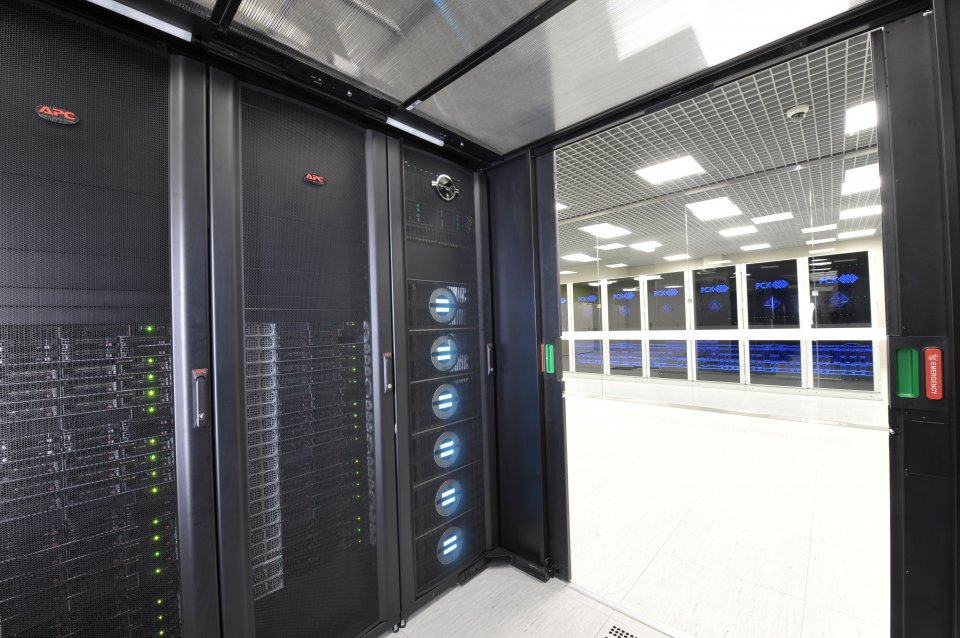
\includegraphics[width=.95\linewidth,valign=t]{my_folder/images/spbpu_sc_system}
	\end{subfigure}
\hfill %выровнять по ширине
	\adjustbox{minipage=1.3em,valign=t}{\subcaption{}\label{fig:spbpu_sc-b}}%
	\begin{subfigure}[t]{\dimexpr.5\linewidth-1.3em\relax}
		\centering
		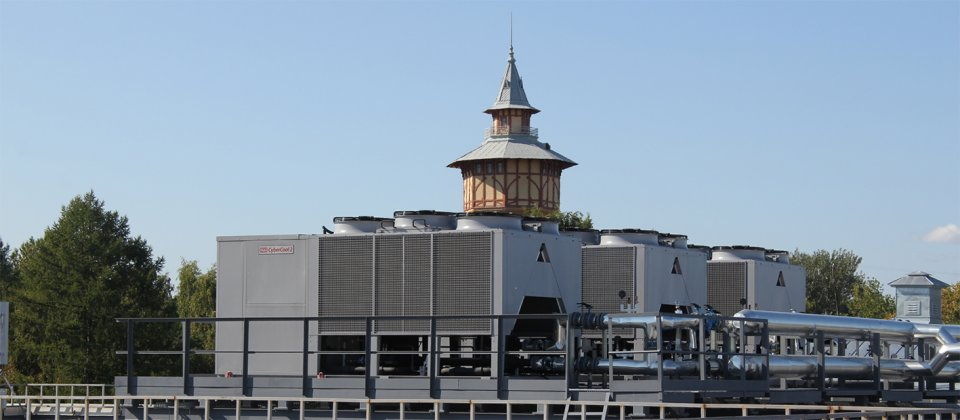
\includegraphics[width=.95\linewidth,valign=t]{my_folder/images/spbpu_sc_refr}
	\end{subfigure}
\\[20pt]
	\adjustbox{minipage=1.3em,valign=t}{\subcaption{}\label{fig:spbpu_sc-c}}%
\begin{subfigure}[t]{\dimexpr.5\linewidth-1.3em\relax}
	\centering
	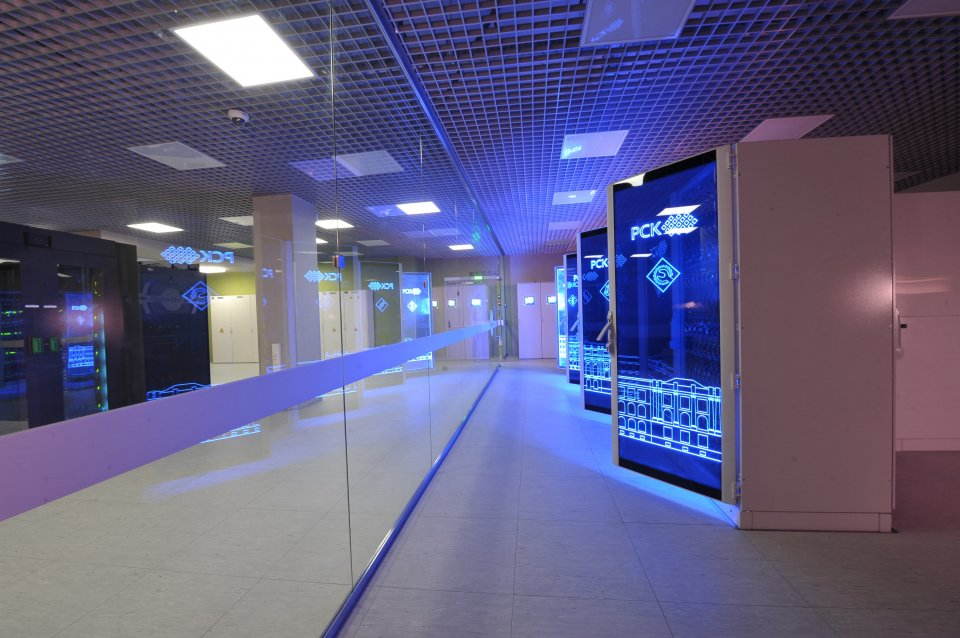
\includegraphics[width=.95\linewidth,valign=t]{my_folder/images/spbpu_sc_hall}
\end{subfigure}%
\hfill %выровнять по ширине
\adjustbox{minipage=1.3em,valign=t}{\subcaption{}\label{fig:spbpu_sc-d}}%
\begin{subfigure}[t]{\dimexpr.5\linewidth-1.3em\relax}
	\centering
	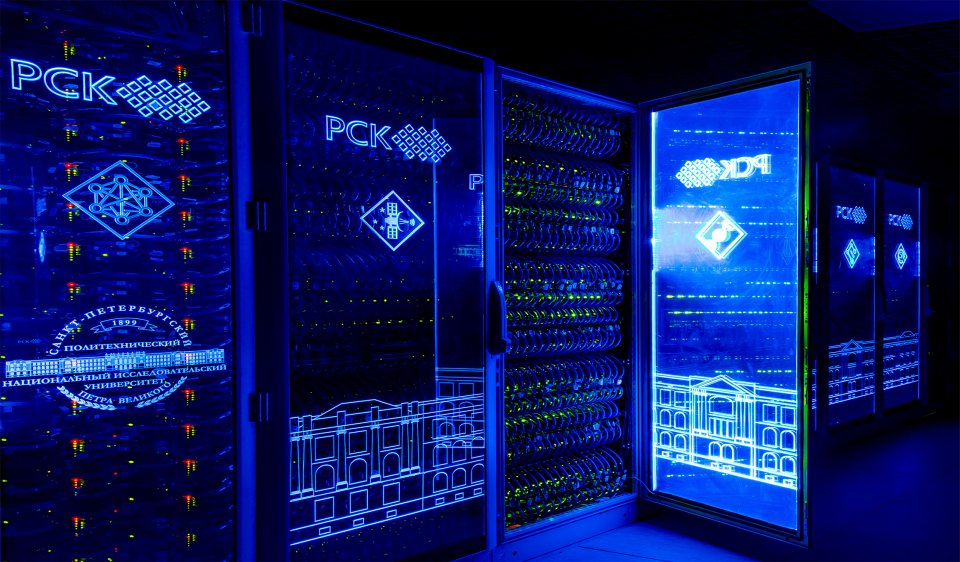
\includegraphics[width=.95\linewidth,valign=t]{my_folder/images/spbpu_sc_box}
\end{subfigure}
\captionsetup{justification=centering} %центрировать
\caption{Фотографии суперкомпьютерного центра СПбПУ \cite{spbpu-gallery}: {\itshape a} --- система хранения данных и узлы NUMA-вычислителя; {\itshape b} --- холодильные машины на крыше научно-исследовательского корпуса; {\itshape c} --- машинный зал; {\itshape d} --- элементы вычислительных устройств} 
\label{fig:spbpu_sc-four-photos}
\end{figure}

Далее можно ссылаться на составные части данного рисунка как на самостоятельные объекты: \firef{fig:spbpu_sc-a}, \firef{fig:spbpu_sc-b}, \firef{fig:spbpu_sc-c}, \firef{fig:spbpu_sc-d} или на три из четырёх изображений одновременно: рис.\labelcref{fig:spbpu_sc-a,fig:spbpu_sc-b,fig:spbpu_sc-c}. % пример подключения 4х иллюстраций в одном рисунке

%На \firef{fig:spbpu_whitehall-three-photos} приведены три картинки под~общим номером и~названием, но с раздельной нумерацией подрисунков посредством пакета \verb|subcaption|.
%
\begin{figure}[!htbp]
	\adjustbox{minipage=1.3em,valign=t}{\subcaption{}\label{fig:spbpu_whitehall-a}}%
	\begin{subfigure}[t]{\dimexpr.3\linewidth-1.3em\relax}
		\centering
		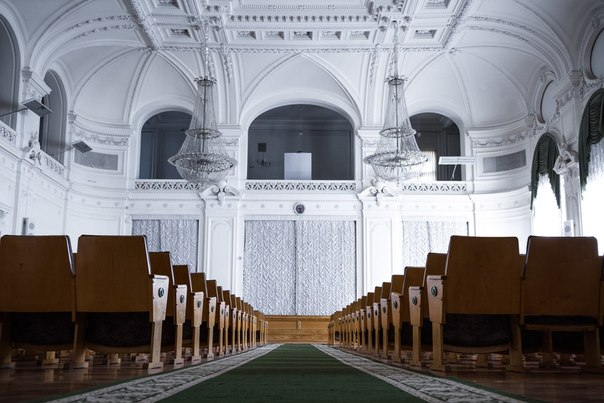
\includegraphics[width=.95\linewidth,valign=t]{my_folder/images//spbpu_whitehall}
	\end{subfigure}
	\hfill %выровнять
	\adjustbox{minipage=1.3em,valign=t}{\subcaption{}\label{fig:spbpu_whitehall-b}}%
	\begin{subfigure}[t]{\dimexpr.3\linewidth-1.3em\relax}
		\centering
		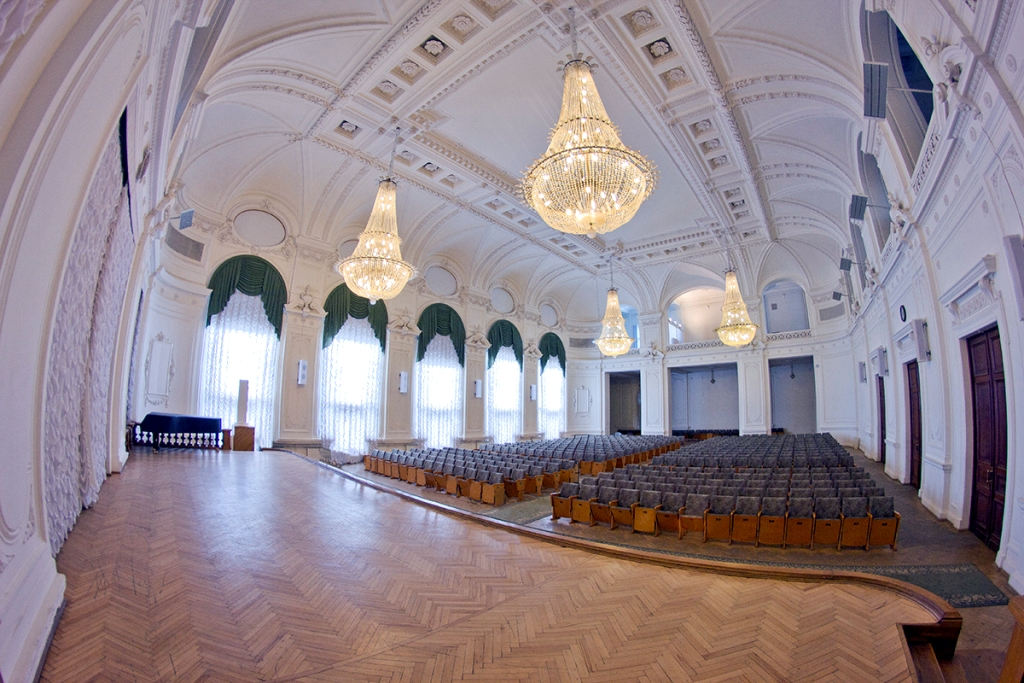
\includegraphics[width=.95\linewidth,valign=t]{my_folder/images//spbpu_whitehall_ligh}
	\end{subfigure}
	\hfill %выровнять
		\adjustbox{minipage=1.3em,valign=t}{\subcaption{}\label{fig:spbpu_whitehall-c}}%
	\begin{subfigure}[t]{\dimexpr.3\linewidth-1.3em\relax}
		\centering
		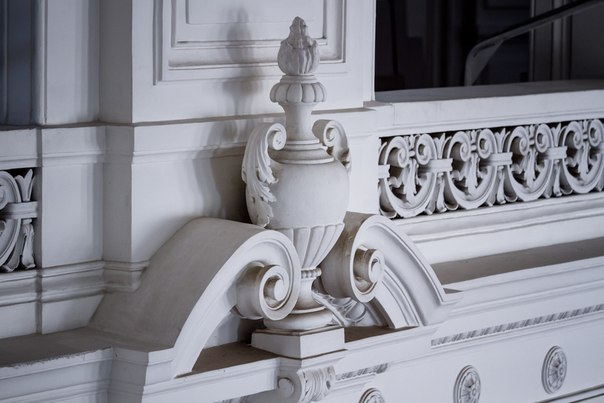
\includegraphics[width=.95\linewidth,valign=t]{my_folder/images//spbpu_whitehall_sculpture}
	\end{subfigure}%
\captionsetup{justification=centering} %центрировать
	\caption{Фотографии Белого зала СПбПУ \cite{spbpu-gallery}, в том числе: {\itshape a} --- со стороны зрителей; {\itshape b} --- со стороны сцены; {\itshape c} --- барельеф}\label{fig:spbpu_whitehall-three-photos}  
\end{figure}

Далее можно ссылаться на три отдельных рисунка: \firef{fig:spbpu_whitehall-a}, \firef{fig:spbpu_whitehall-b} и \firef{fig:spbpu_whitehall-c}. % пример подключения 3х иллюстрации в одном рисунке
%
%На \firef{fig:spbpu_main_bld-two-photos} приведены две картинки под~общим номером и~названием.


\begin{figure}[!htbp]
	\adjustbox{minipage=1.3em,valign=t}{\subcaption{}\label{fig:spbpu_main_bld_entrance_autumn}}%
	\begin{subfigure}[t]{\dimexpr.5\linewidth-1.3em\relax} %разрешили выделить 0,5 стр в ширину на рисунок
		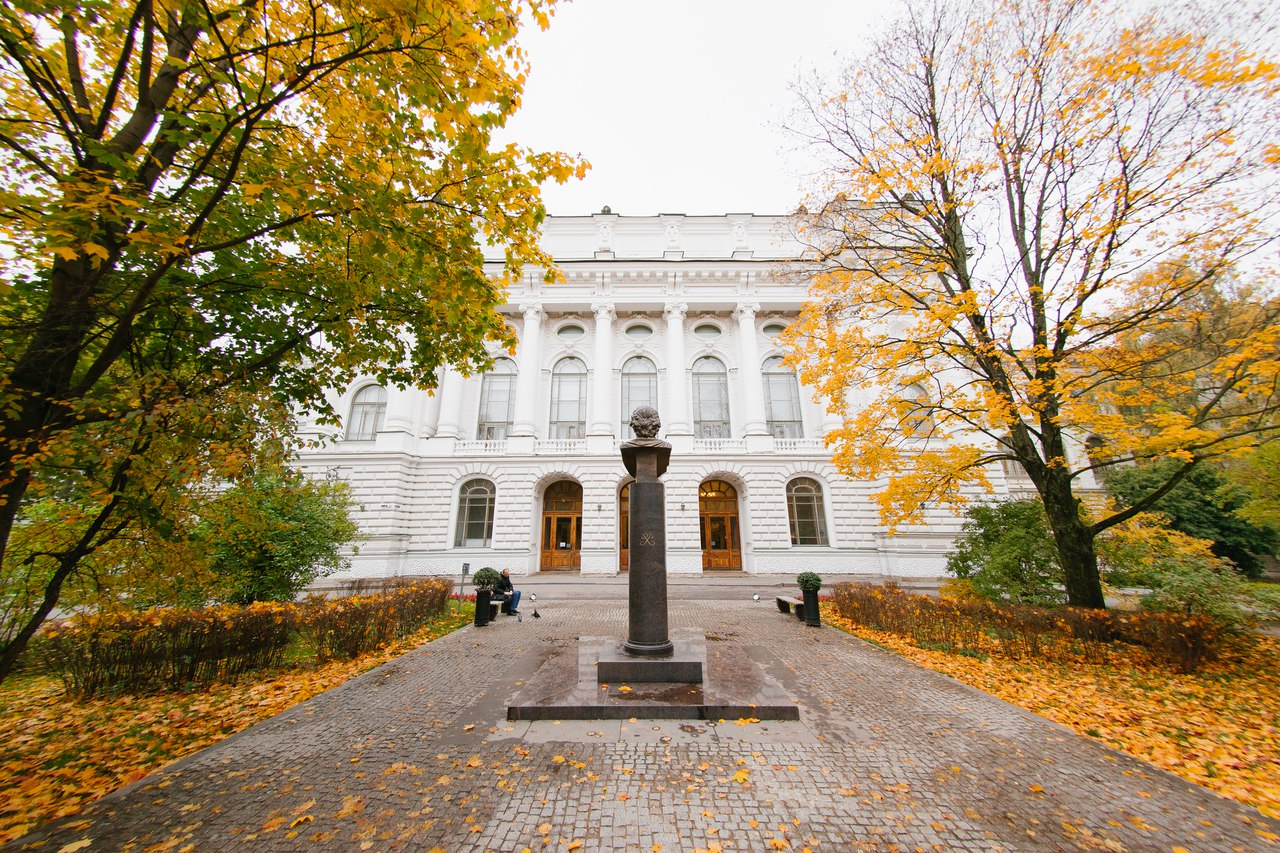
\includegraphics[height=0.20\textheight,valign=t]{my_folder/images//spbpu_main_bld_entrance_autumn} %высоту рисунка выставили как 0,3 от высоты наборного поля
	\end{subfigure}
%	\hfill %выровнять по ширине
	\adjustbox{minipage=1.3em,valign=t}{\subcaption{}\label{fig:spbpu_main_bld_whitehall}}%
	\begin{subfigure}[t]{\dimexpr.5\linewidth-1.3em\relax}%разрешили выделить 0,5 стр в ширину на рисунок
		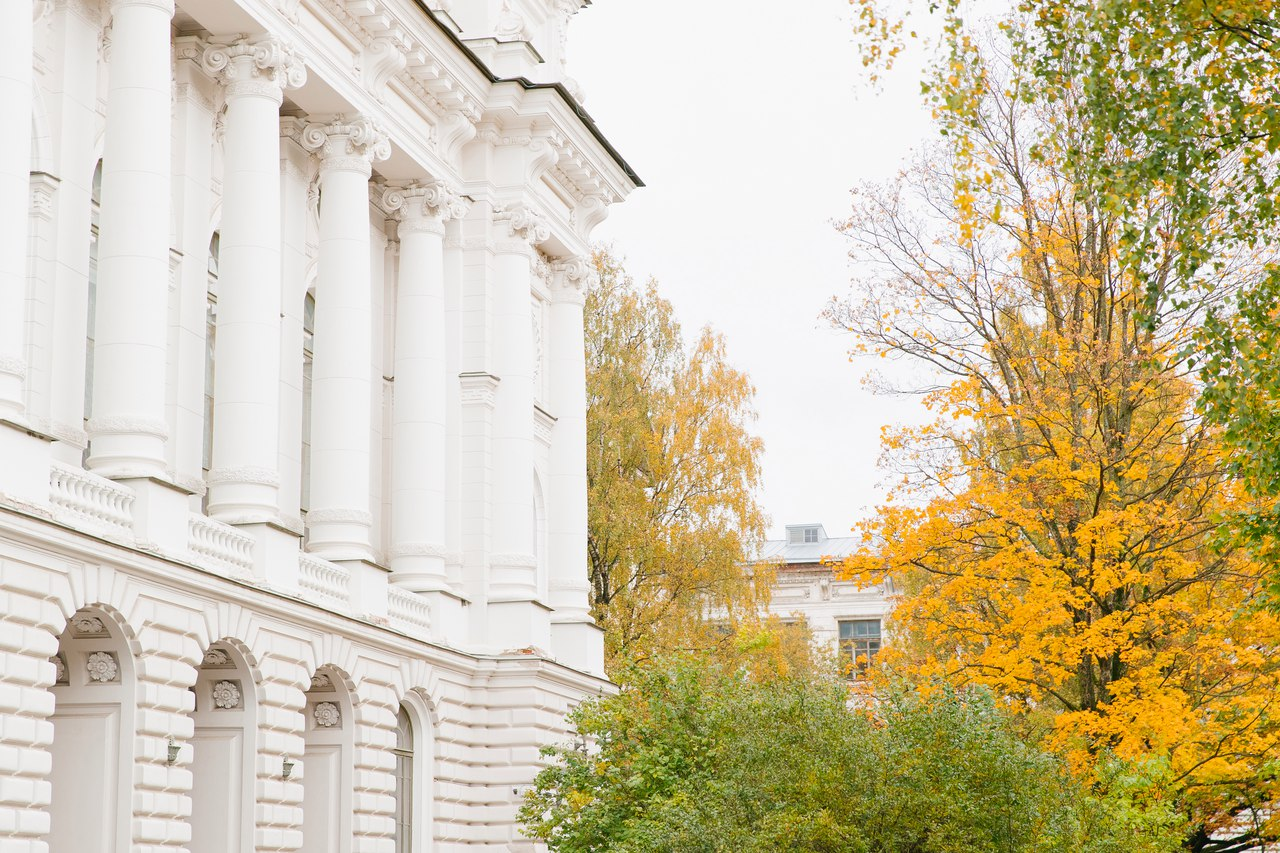
\includegraphics[height=0.20\textheight,valign=t]{my_folder/images//spbpu_main_bld_whitehall}%высоту рисунка выставили как 0,3 от высоты наборного поля
	\end{subfigure}
\captionsetup{justification=centering} %центрировать
	\caption{Вид на главное здание СПбПУ \cite{spbpu-gallery}, включая: {\itshape a} --- вход со стороны парка осенью; {\itshape b}~--- окна Белого зала}\label{fig:spbpu_main_bld-two-photos} 
\end{figure}

На \firef{fig:spbpu_main_bld_entrance_autumn} изображен вход со стороны парка СПбПУ осенью, а на \firef{fig:spbpu_main_bld_whitehall}~--- окна Белого зала. % пример подключения 2х иллюстраций в одном рисунке

Приведём пример табличного представления данных с записью продолжения на следующей странице на \taref{tab:long}.

%%% отладка longtable
%% 1) для контроля выхода таблицы за границы полей выставляем showframe в \geometry{}, см настройки
%% 2) используем \\* для запрета переноса определенной строки или средства из:
%% https://tex.stackexchange.com/q/344270/44348
%% 3) в крайнем случае для принудительного переноса таблицы на новую страницу используем \pagebreak после \\
\noindent % for correct centering
\begingroup
\centering
\small %выставляем шрифт в 12bp
\begin{longtable}[c]{|l|l|l|l|l|l|}
	\caption{Пример задания данных из \cite{Peskov2004} (с повтором для переноса таблицы на новую страницу)}%
	\label{tab:long}% label всегда желательно идти после caption
	\\
	\hline
	$G$&$m_1$&$m_2$&$m_3$&$m_4$&$K$\\ \hline
	1&2&3&4&5&6\\ \hline
	\endfirsthead%
	\captionsetup{format=tablenocaption,labelformat=continued} % до caption!
	\caption[]{}\\ % печать слов о продолжении таблицы
	\hline
	1&2&3&4&5&6\\ \hline
	\endhead
	\hline
	\endfoot
	\hline
	\endlastfoot
	$g_1$&0&1&1&0&1\\ \hline
	$g_2$&1&2&0&1&1\\ \hline
	$g_3$&0&1&0&1&1\\ \hline
	$g_4$&1&2&1&0&2\\ \hline
	$g_5$&1&1&0&1&2\\ \hline
	$g_6$&1&1&1&2&2\\ \hline
%
	$g_1$&0&1&1&0&1\\ \hline 
	$g_2$&1&2&0&1&1\\ \hline
	$g_3$&0&1&0&1&1\\ \hline
	$g_4$&1&2&1&0&2\\ \hline \noalign{\penalty-5000} % способствуем переносу на следующую стр
	$g_5$&1&1&0&1&2\\ \hline 
	$g_6$&1&1&1&2&2\\ \hline
%
	$g_1$&0&1&1&0&1\\ \hline 
	$g_2$&1&2&0&1&1\\ \hline
	$g_3$&0&1&0&1&1\\ \hline
	$g_4$&1&2&1&0&2\\ \hline
	$g_5$&1&1&0&1&2\\ \hline
	$g_6$&1&1&1&2&2\\ \hline
%		
	$g_1$&0&1&1&0&1\\ \hline 
	$g_2$&1&2&0&1&1\\ \hline
	$g_3$&0&1&0&1&1\\ \hline
	$g_4$&1&2&1&0&2\\ \hline
	$g_5$&1&1&0&1&2\\ \hline
	$g_6$&1&1&1&2&2\\ \hline
%
	$g_1$&0&1&1&0&1\\ \hline 
	$g_2$&1&2&0&1&1\\ \hline
	$g_3$&0&1&0&1&1\\ \hline
	$g_4$&1&2&1&0&2\\ \hline
	$g_5$&1&1&0&1&2\\ \hline
	$g_6$&1&1&1&2&2\\ \hline
%
	$g_1$&0&1&1&0&1\\ \hline 
	$g_2$&1&2&0&1&1\\ \hline
	$g_3$&0&1&0&1&1\\ \hline
	$g_4$&1&2&1&0&2\\ \hline
	$g_5$&1&1&0&1&2\\ \hline
	$g_6$&1&1&1&2&2\\ \hline
%
	$g_1$&0&1&1&0&1\\ \hline 
	$g_2$&1&2&0&1&1\\ \hline
	$g_3$&0&1&0&1&1\\ \hline
	$g_4$&1&2&1&0&2\\ \hline
	$g_5$&1&1&0&1&2\\ \hline
	$g_6$&1&1&1&2&2\\ \hline
\end{longtable}
\normalsize% возвращаем шрифт к нормальному
\endgroup % пример подключения таблицы на несколько страциц


\begin{table} [htbp]% Пример оформления таблицы
	\centering\small
	\caption{Пример представления данных для сквозного примера по ВКР \cite{Peskov2004}}%
	\label{tab:ToyCompare}		
		\begin{tabular}{|l|l|l|l|l|l|}
			\hline
			$G$&$m_1$&$m_2$&$m_3$&$m_4$&$K$\\
			\hline
			$g_1$&0&1&1&0&1\\ \hline
			$g_2$&1&2&0&1&1\\ \hline
			$g_3$&0&1&0&1&1\\ \hline
			$g_4$&1&2&1&0&2\\ \hline
			$g_5$&1&1&0&1&2\\ \hline
			$g_6$&1&1&1&2&2\\ \hline		
		\end{tabular}
%	\caption*{\raggedright\hspace*{2.5em} Составлено (или/и рассчитано) по \cite{Peskov2004}} %Если проведена авторская обработка или расчеты по какому-либо источнику	
	\normalsize% возвращаем шрифт к нормальному
\end{table}



%% please, before using, read the author guide carefully

\noindent % for correct centering
\begin{minipage}{\textwidth}
	\vspace{\mfloatsep} % интервал 
	\centering\small
	\captionof{table}{Пример задания данных в табличном виде из \cite{Peskov2004} (с помощью окружения minipage)}%
	\label{tab:ToyCompare-Peskov-minipage}
	\begin{tabular}{|l|l|l|l|l|l|}
	\hline
	$G$&$m_1$&$m_2$&$m_3$&$m_4$&$K$\\
	\hline
	$g_1$&0&1&1&0&1\\ \hline
	$g_2$&1&2&0&1&1\\ \hline
	$g_3$&0&1&0&1&1\\ \hline
	$g_4$&1&2&1&0&2\\ \hline
	$g_5$&1&1&0&1&2\\ \hline
	$g_6$&1&1&1&2&2\\ \hline
	\hline		
	\end{tabular}
\vspace{\mfloatsep} % интервал 
\normalsize %восстанавливаем шрифт 	
\end{minipage} % пример подключения minipage

\noindent % for correct centering
\begin{minipage}{\textwidth}
	\centering
	\vspace{\mfloatsep} % интервал  	
	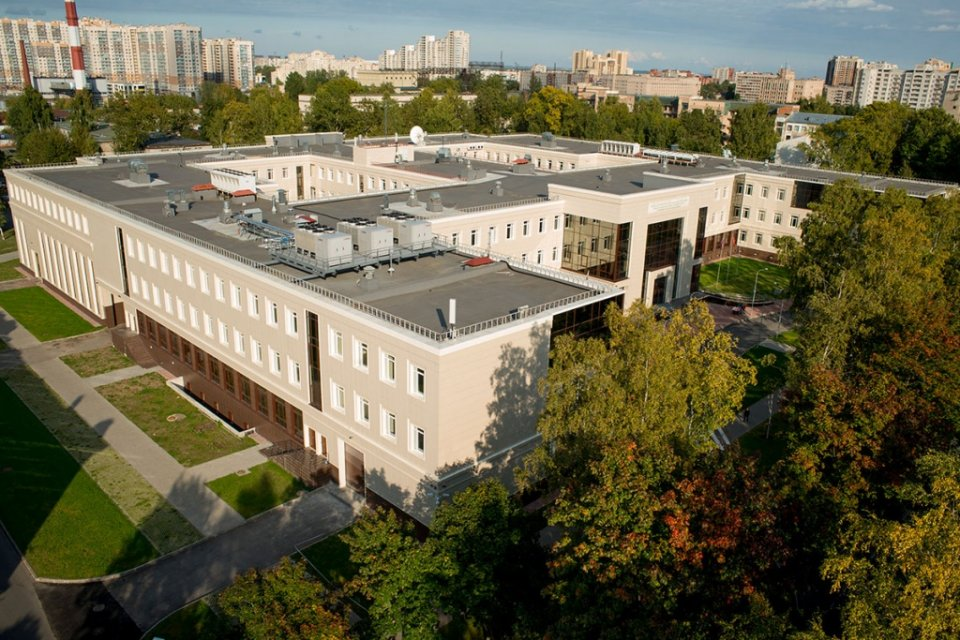
\includegraphics[keepaspectratio=true,scale=0.27] {my_folder/images/spbpu_new_bld_autumn}
	\captionof{figure}{Новый научно-исследовательский корпус СПбПУ \cite{spbpu-gallery} (с помощью окружения minipage)}\label{fig:spbpu-new-bld-autumn-minipage}  
	\vspace{\mfloatsep} % интервал  	
\end{minipage} % пример подключения minipage




Вопросы форматирования текстово-графических объектов (окружений) не регламентированы в известных нам ГОСТах, поэтому предлагаем придерживаться следующих правил:

\begin{itemize}
	\item \textbf{полужирный текст} рекомендуем использовать только для названий стандартных окружений с нумерационной частью, например, для представления \textit{впервые}: \textbf{определение 1.1}, \textbf{теорема 2.2}, \textbf{пример 2.3}, \textbf{лемма 4.5};
	
	\item \textit{курсив} рекомендуем использовать только для выделения переменных в формулах, служебной информации об авторах главы (статьи), важных терминов, представляемых по тексту, а также для всего тела окружений, связанных с получением \textit{новых существенных результатов и их доказательством}: теорема, лемма, следствие, утверждение и другие.
\end{itemize}

 

По аналогии с нумерацией формул, рисунков и таблиц нумеруются и иные текстово-графические объекты, то есть включаем в нумерацию номер главы, например: теорема 3.1. для первой теоремы третьей главы монографии. Команды \LaTeX{} выставляют нумерацию и форматирование автоматически. Полный перечень команд для подготовки текстово-графических и иных объектов находится в подробных методических рекомендациях \cite{spbpu-bci-template-author-guide}. 


Для удобства авторов названия стандартных окружений, рекомендованных к использованию, приведены в \taref{tab:enum-std}, а в \taref{tab:enum-spbpu}  перечислены имена специально разработанных окружений для шаблонов SPbPU.

% и примеры их оформления на псевдокоде (см. \cite{cite-spbpu-bci}).


%https://tex.stackexchange.com/questions/2651/should-i-use-center-or-centering-for-figures-and-tables


	\begin{table} [htbp]% Пример записи таблицы с номером, но без отображаемого наименования
	\centering\small
	\caption{Стандартные окружения}%
	\label{tab:enum-std}
	 \begin{Spacing}{\Single} % Одинарный интервал между строками текста 
	  \renewcommand*{\arraystretch}{1.5} % Полуторный интервал между ячейками таблицы
		\begin{tabular}{|l|p{11cm}|} 
			\hline
			Название окружения&Назначение\\
			\hline
			\verb|center| &	центрирование, аналог команды \verb|\centering|, но с добавлением нежелательного пробела, поэтому лучше избегать применения \verb|center|\\ \hline
			\verb|itemize| &{перечисления, в которых нет необходимости нумеровать  пункты (немаркированные списки)} \\ \hline
			\verb|enumerate| & перечисления с нумерацией (немаркированные списки) \\ \hline
			\verb|refsection| & создание отдельных библиографических списков для глав \\ \hline
			\verb|tabular| & оформление таблиц \\ \hline
			\verb|table|   &{автоматическое перемещение по тексту таблиц, оформленных, например, с помощью \verb|tabular|, для минимизации пустых пространств} \\ \hline
			\verb|longtable| & оформление многостраничных таблиц \\ \hline
			\verb|tikzpicture| & создание иллюстраций с помощью пакета \verb|tikz| \cite{ctan-tikz} \\ \hline
			\verb|figure| &{автоматическое перемещение по тексту рисунков, оформленных например, с помощью \verb|tikz| или подключенных с помощью команды \verb|\includegraphics|, для минимизации пустых пространств} \\ \hline 
			\verb|subfigure| & оформление вложенных рисунков в составе \verb|figure| \\ \hline
			\verb|algorithm| &{оформление псевдокода на основе пакета \verb|algorithm2e| \cite{ctan-algorithm2e}} \\ \hline
			\verb|minipage| & {оформление рисунков и таблиц без функций автоматического перемещения по тексту для  минимизации пустых пространств} \\ \hline
			\verb|equation| & {оформление выключенных (не встроенных в текст с помощью \verb|$...$|) одиночных формул на одной строке} \\ \hline
			\verb|multilined| &{оформление выключенных (не встроенных в текст с помощью \verb|$...$|) одиночных формул в несколько строк} \\ \hline 
			\verb|aligned| &{оформление нескольких формул с выравниванием по символу \verb|&|.} \\ \hline
	\end{tabular}
	\end{Spacing}
%	\normalsize
	\end{table}

На базе пакета \verb|tikz| разработано большое количество расширений \cite{ctan-tikz}, например, \verb|tikzcd|, которые мы рекомендуем использовать для оформления иллюстраций.

	\begin{table} [htbp]% Пример записи таблицы с номером, но без отображаемого наименования
	\centering\small
	\caption{Специальные окружения}%
	\label{tab:enum-spbpu}
		\begin{tabular}{|l|l|}
			\hline
			Название окружения & Текстово-графический объект\\
			\hline
			\verb|abstr|	 & реферат (abstract) \\ \hline
			\verb|m-theorem| & теорема \\ \hline 
			\verb|m-corollary| & следствие \\ \hline
			\verb|m-proposition| & утверждение \\ \hline
			\verb|m-lemma|   & лемма \\ \hline
			\verb|m-axiom| & аксиома \\ \hline
			\verb|m-example| & пример \\ \hline
			\verb|m-definition| &  определение \\ \hline
			\verb|m-condition| & условие \\ \hline
			\verb|m-problem| & проблема \\ \hline
			\verb|m-exercise| & упраженение \\ \hline
			\verb|m-question| & вопрос \\ \hline
			\verb|m-hypothesis| & гипотеза \\ \hline
		\end{tabular}	
	\normalsize
\end{table}

В случае, если авторам потребовалось новое окружение, то создать его можно в файле в файле \texttt{my\_fol\-der/{}my\_set\-tings.tex} согласно правилам, приведённым ниже.

\begin{enumerate}[1.]
	\item Для перехода в режим создания окружений следует указать:
	\begin{itemize}
		\item \verb|\theoremstyle{myplain}| --- окружения с доказательствами или аксиомами
		\item \verb|\theoremstyle{mydefinition}| --- окружения, не связанные с доказательствами или аксиомами.
	\end{itemize}
	\item В команде создания окружения следует ввести краткий псевдоним (\verb|m-new-env|) и отображаемое в pdf имя окружения (\verb|Название_окружения|):
	\begin{itemize}
		\item \texttt{\textbackslash{}newtheorem\{m-new-env-second\}\{Название\_окруже\-ния\}\-[chap\-ter]}.
	\end{itemize}
\end{enumerate}


%\begin{m-new-env-first}
%	Тест первого пользовательского окружения
%\end{m-new-env-first}
%
%\begin{m-new-env-second}
%	Тест второго пользовательского окружения
%\end{m-new-env-second} % список некоторых окружений


\begin{m-theorem}[о чем-то конкретном] %при необходимости в [] можно записать название теоремы или убрать его
	\label{th:ex} 
	% \index только для принятых работ
	% шаблон записи теоремы в Предметный указатель
	\index[ru]{теорема!название\_теоремы или о чём} %ключевое слово <<теорема>> не менять
	\index[en]{theorem!1-3 words for detail or description}
	% пример записи алгоритма в Предметный указатель
	\index[ru]{теорема!о неполноте}
	\index[en]{theorem!about incompleteness}
	% пример записи алгоритма в Предметный указатель
	\index[ru]{теорема!о жизни}
	\index[en]{theorem!about life}
	Текст теоремы полностью выделен курсивом. Допустимо математические символы не выделять курсивом, если это искажает их значения. Используется абзацный отсуп, так как ``Абзацы в тексте начинают отступом'' в соответствии с ГОСТ 2.105--95. Название теоремы допустимо убрать. Доказательство окончено.
\end{m-theorem}
Доказательство теоремы \ref{th:ex}, леммы, утверждений, следствий и других подобных окружений (в последнем абзаце) завершаем предложением в котором сказано, что доказательство окончено. Например, доказательство теоремы \ref{th:ex} окончено.

Тело доказательства не выделяется курсивом.
Тело следующих окружений также не выделяется сплошным курсивом: определение, условие, проблема, пример, упражнение, вопрос, гипотеза и другие. %пример оформления теоремы


\begin{m-definition}[термин] %при необходимости в [] можно записать название определения или убрать его
	\label{def:ex}
	% \index только для принятых работ
	% шаблон записи определения в Предметный указатель 
	\index[ru]{название\_определения!1-3 уточняющих слова или~ничего}
	\index[en]{definition\_title!1-3 words for detail or~without "!-part}
	% пример записи определения в Предметный указатель 
	\index[ru]{и-тест!хороший!наилучший}
	\index[en]{i-test!good!best}
	% пример записи определения в Предметный указатель 
	\index[ru]{и-тест!замкнутый}
	\index[en]{i-test!closed}
	В тексте определения только {\itshape важные термины} выделяются курсивом. Если определение носит лишь вспомогательный характер, то допустимо не использовать окружение \texttt{m-definition}, представляя текст определения в обычном абзаце. Ключевые термины при этом обязательно выделяются курсивом.
\end{m-definition} %пример оформления определения


Вместо теоремо-подобных окружений для вставки небольших текстово-графических объектов иногда используются команды. Типичным примером такого подхода является команда \verb|\footnote{text}|\footnote{Внимание! Команда вставляется непосредственно после слова, куда вставляется сноска (без пробела). Лишние пробелы также не указываются внутри команды перед и после фигурных скобок.}, где в аргументе \verb|text| указывают текст \textit{подстрочной ссылки (сноски)}.В них \textit{нельзя добавлять веб-ссылки или цитировать литературу}. Для этих целей используется список литературы. Нумерация сносок сквозная по ВКР без точки на конце выставляется в шаблоне автоматически, однако в каждом приложении к ВКР нумерация, зависящая от номера приложения, выставляется префикс <<П>>, например <<П1.1>> --- первая сноска первого приложения. 




%\FloatBarrier % заставить рисунки и другие подвижные (float) элементы остановиться


\section{Выводы} \label{ch2:conclusion}

Текст заключения ко второй главе. Пример ссылок \cite{Article,Book,Booklet,Conference,Inbook,Incollection,Manual,Mastersthesis,Misc,Phdthesis,Proceedings,Techreport,Unpublished,badiou:briefings}, а также ссылок с указанием страниц, на котором отображены те или иные текстово-графические объекты  \cite[с.~96]{Naidenova2017} или в виде мультицитаты на несколько источников \cites[с.~96]{Naidenova2017}[с.~46]{Ganter1999}. Часть библиографических записей носит иллюстративный характер и не имеет отношения к реальной литературе. 

Короткое имя каждого библиографического источника содержится в специальном файле \verb|my_biblio.bib|, расположенном в папке \verb|my_folder|. Там же находятся исходные данные, которые с помощью программы \texttt{Biber} и стилевого файла \texttt{Biblatex-GOST} \cite{ctan-biblatex-gost} приведены в списке использованных источников согласно ГОСТ 7.0.5-2008.
Многообразные реальные примеры исходных библиографических данных можно посмотреть по ссылке \cite{ctan-biblatex-gost-examples}.

Как правило, ВКР должна состоять из четырех глав. Оставшиеся главы можно создать по образцу первых двух и подключить с помощью команды \verb|\input| к исходному коду ВКР. Далее в приложении \ref{appendix-MikTeX-TexStudio} приведены краткие инструкции запуска исходного кода ВКР \cite{latex-miktex,latex-texstudio}.

В приложении \ref{appendix-extra-examples} приведено подключение некоторых текстово-графических объектов. Они оформляются по приведенным ранее правилам. В качестве номера структурного элемента вместо номера главы используется <<П>> с номером главы. Текстово-графические объекты из приложений не учитываются в реферате.



%% Вспомогательные команды - Additional commands
%
%\newpage % принудительное начало с новой страницы, использовать только в конце раздела
%\clearpage % осуществляется пакетом <<placeins>> в пределах секций
%\newpage\leavevmode\thispagestyle{empty}\newpage % 100 % начало новой страницы